\documentclass[a4paper,11pt]{article}
\usepackage{graphicx}
\usepackage{amsmath}
\usepackage{hyperref}
\usepackage{geometry}
\usepackage{subcaption}
\usepackage[francais]{babel}
\geometry{left=2.0cm,right=2.0cm,top=2.5cm,bottom=2.5cm}
% \captionsetup{compatibility=true}
\title{Rapport Jalon 2}
\author{\textbf{Benjamin PELLIEUX}}
\date{\today}

\begin{document}

\maketitle
\section{Jalon 2 : Simulation de la conduction thermique en régime transitoire}

\subsection{Problématique générale}
La problématique reste identique à celle présentée pour le Jalon 1. Il s'agit de comprendre la diffusion de la chaleur à travers un mur en béton, en modélisant la conduction thermique. L'objectif global est de réduire les coûts de chauffage tout en assurant un confort thermique optimal pour les occupants du bâtiment.

\subsection{Objectifs du Jalon 2}
L'objectif de ce jalon est de modéliser la conduction thermique en \textbf{régime transitoire} dans un mur en béton, en tenant compte de l'évolution de la température au fil du temps. Contrairement au Jalon 1 qui se concentrait sur le régime stationnaire, ce jalon vise à observer l'évolution de la température sur une période de 96 heures. Deux scénarios de conditions aux limites sont simulés :
\begin{itemize}
    \item \textbf{Dirichlet-Dirichlet} : Températures imposées aux deux extrémités du mur.
    \item \textbf{Dirichlet-Neumann} : Température imposée à une extrémité et flux thermique nul à l'autre.
\end{itemize}
Un terme de source de chaleur est ajouté au centre du mur pour simuler un apport thermique supplémentaire.

\subsection{Méthodologie}
Pour résoudre l'équation de la chaleur en régime transitoire, nous utilisons une approche discrétisée à l'aide de la \textbf{méthode des volumes finis (MVF)}. La discrétisation spatiale est effectuée en découpant le mur en 1000 volumes finis, tandis que la discrétisation temporelle est réalisée avec un pas de temps de 15 minutes (\(dt = 900 \, s\)). La simulation s'étend sur une période de 96 heures (\(t_{\text{total}} = 3600 \times 96 \, s\)).

Les hypothèses principales sont les suivantes :
\begin{itemize}
    \item Le mur est modélisé comme un milieu homogène avec une conductivité thermique \(k = 1.5 \, W/m \cdot K\).
    \item Les variations de température au sein du mur sont modélisées en fonction de la position et du temps.
    \item La chaleur est diffusée à travers le mur, avec une source de chaleur au centre pour simuler un apport énergétique constant.
\end{itemize}

La résolution du système d'équations est effectuée à l'aide de la fonction \texttt{solve\_banded} de \texttt{scipy}, adaptée à la structure tridiagonale de la matrice de coefficients. Les conditions aux limites sont intégrées directement dans la matrice de coefficients avant chaque résolution.
\subsection{Résultats}
La simulation produit des graphiques 3D illustrant la \textbf{distribution de la température} dans le mur en fonction de la \textbf{position} et du \textbf{temps}. Les résultats montrent comment la température évolue sur 96 heures et 128 heures, permettant d'observer la propagation de la chaleur dans le mur au fil du temps.

\begin{figure}[!ht]
    \centering
    \begin{subfigure}{0.45\textwidth}
        \centering
        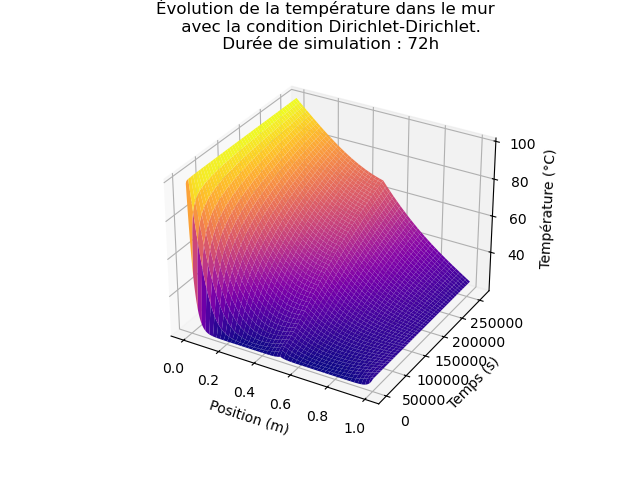
\includegraphics[width=\textwidth]{img/Figure_DD_3D.png} % Remplacer par le chemin vers votre image
        \caption{96H, Dirichlet-Dirichlet.}
        \label{fig:jalon2_dirichlet_dirichlet_96H}
    \end{subfigure}
    \hfill
    \begin{subfigure}{0.45\textwidth}
        \centering
        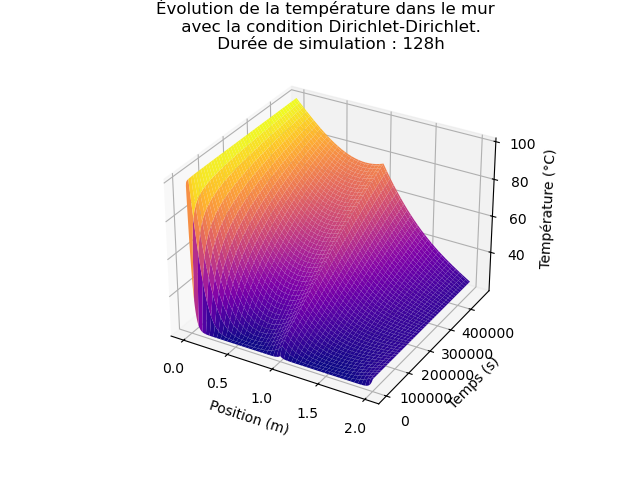
\includegraphics[width=\textwidth]{img/Figure_DD_3D_128.png} % Remplacer par le chemin vers votre image
        \caption{128H, Dirichlet-Dirichlet.}
        \label{fig:jalon2_dirichlet_dirichlet_128H}
    \end{subfigure}
    \caption{Comparaison de l'évolution de la température dans le mur avec la condition Dirichlet-Dirichlet entre 96H et 128H.}
    \label{fig:jalon2_comparaison_dirichlet_dirichlet}
\end{figure}

\begin{figure}[!ht]
    \centering
    \begin{subfigure}{0.45\textwidth}
        \centering
        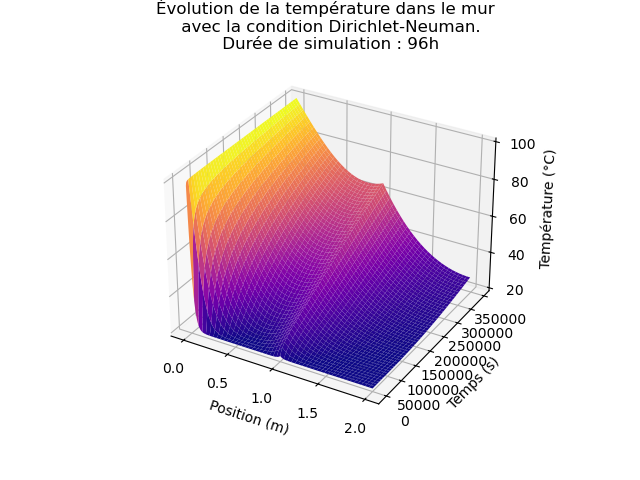
\includegraphics[width=\textwidth]{img/Figure_DN_3D.png} % Remplacer par le chemin vers votre image
        \caption{96H, Dirichlet-Neumann.}
        \label{fig:jalon2_dirichlet_neumann_96H}
    \end{subfigure}
    \hfill
    \begin{subfigure}{0.45\textwidth}
        \centering
        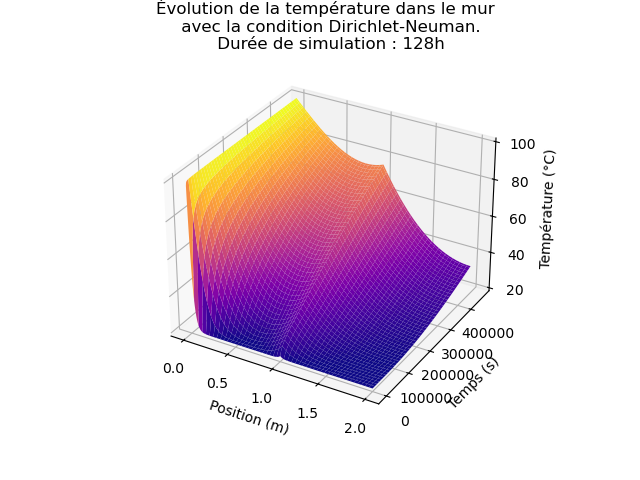
\includegraphics[width=\textwidth]{img/Figure_DN_3D_128.png} % Remplacer par le chemin vers votre image
        \caption{128H, Dirichlet-Neumann.}
        \label{fig:jalon2_dirichlet_neumann_128H}
    \end{subfigure}
    \caption{Comparaison de l'évolution de la température dans le mur avec la condition Dirichlet-Neumann entre 96H et 128H.}
    \label{fig:jalon2_comparaison_dirichlet_neumann}
\end{figure}

\subsection{Analyse des résultats}
Les graphiques présentés aux figures \ref{fig:jalon2_dirichlet_dirichlet_96H}, \ref{fig:jalon2_dirichlet_dirichlet_128H}, \ref{fig:jalon2_dirichlet_neumann_96H} et \ref{fig:jalon2_dirichlet_neumann_128H} montrent l'évolution de la température dans un mur de béton en fonction de la position et du temps pour deux types de conditions aux limites (Dirichlet-Dirichlet et Dirichlet-Neumann) et pour deux durées de simulation (96 heures et 128 heures).

\subsubsection{Analyse du scénario Dirichlet-Dirichlet}
\begin{itemize}
    \item \textbf{96 heures (Figure \ref{fig:jalon2_dirichlet_dirichlet_96H}) :} La température est initialement plus élevée du côté gauche, où la température est fixée à 100°C, et diminue progressivement vers la droite, où la température est fixée à 25°C. Après 96 heures, la courbe montre que la chaleur continue de se diffuser mais tend à se stabiliser, indiquant que l'équilibre thermique est presque atteint.
    \item \textbf{128 heures (Figure \ref{fig:jalon2_dirichlet_dirichlet_128H}) :} En prolongeant la simulation à 128 heures, on observe que la température se stabilise davantage, atteignant un état proche de l'équilibre. Le gradient de température devient plus régulier, ce qui montre que le mur a presque atteint un équilibre thermique global entre les deux extrémités.
\end{itemize}

\subsubsection{Analyse du scénario Dirichlet-Neumann}
\begin{itemize}
    \item \textbf{96 heures (Figure \ref{fig:jalon2_dirichlet_neumann_96H}) :} La température décroît depuis le côté gauche (100°C) vers l'intérieur du mur, mais le profil de température est moins linéaire en raison de la condition de flux nul à droite. La chaleur se dissipe plus lentement vers l'extrémité droite, ce qui se traduit par un plateau thermique vers la fin de la simulation.
    \item \textbf{128 heures (Figure \ref{fig:jalon2_dirichlet_neumann_128H}) :} À 128 heures, l'évolution montre que la température a continué à se diffuser, mais le flux nul à droite maintient une température légèrement plus élevée sur cette partie du mur. Le plateau thermique reste visible, indiquant que la dissipation de la chaleur est plus lente à l'extrémité où le flux est nul.
\end{itemize}

\subsubsection{Comparaison entre 96H et 128H}
\begin{itemize}
    \item En comparant les résultats à 96 heures et 128 heures, on constate que les différences se situent principalement dans la stabilisation des températures. L'augmentation du temps de simulation permet au système de se rapprocher de l'équilibre thermique, en particulier dans le cas Dirichlet-Dirichlet.
    \item Pour le scénario Dirichlet-Dirichlet, l'allongement de la durée de simulation réduit le gradient thermique entre les extrémités du mur, ce qui indique une diffusion continue de la chaleur vers un état homogène.
    \item Dans le cas Dirichlet-Neumann, l'effet de la condition de flux nul est plus marqué avec le temps, montrant une tendance à conserver davantage de chaleur sur la partie droite du mur. Cela confirme que le flux nul agit comme une barrière à la dissipation de la chaleur.
\end{itemize}


\subsection{Conclusion}
Les simulations réalisées dans le cadre du Jalon 2 ont permis de modéliser et d'analyser la diffusion de la chaleur à travers un mur en béton en régime transitoire, en prenant en compte différentes conditions aux limites (Dirichlet-Dirichlet et Dirichlet-Neumann) et des durées de simulation prolongées (96 heures et 128 heures). 

Les résultats montrent que le choix des conditions aux limites a un impact significatif sur la manière dont la chaleur se dissipe au fil du temps :
\begin{itemize}
    \item Le scénario \textbf{Dirichlet-Dirichlet} tend vers un équilibre thermique plus rapide, où le gradient de température devient homogène à mesure que le temps de simulation augmente.
    \item Le scénario \textbf{Dirichlet-Neumann} conserve davantage de chaleur à l'extrémité où le flux est nul, créant un plateau thermique qui persiste même avec une simulation prolongée.
\end{itemize}

La comparaison entre les durées de 96 heures et 128 heures a également mis en lumière l'importance de la durée de simulation pour observer la stabilisation des températures dans le mur. L'allongement de la durée de simulation permet d'approcher plus fidèlement l'état d'équilibre thermique, particulièrement dans le cas des conditions Dirichlet-Dirichlet.

Ces analyses soulignent la nécessité de prendre en compte la dynamique temporelle dans la conception de systèmes de gestion thermique. Elles permettent de mieux comprendre le comportement d'un matériau dans des conditions réalistes de chauffage, offrant des perspectives pour l'optimisation de la consommation énergétique dans les bâtiments. Le prochain jalon se concentrera sur l'optimisation des cycles de chauffage pour maximiser l'efficacité énergétique tout en maintenant un confort thermique adapté aux besoins des occupants.

\end{document}